\documentclass[12pt,a4paper]{article}
\usepackage{amsmath, amssymb, geometry, booktabs, xcolor, hyperref,
            listings, pgfplots, tcolorbox, fancyhdr, tikz, array}
\usepackage[shortlabels]{enumitem}
\geometry{margin=2.5cm}
\setlength{\headheight}{14.5pt}
\pgfplotsset{compat=1.18}
\tcbuselibrary{skins, breakable}

% ---- tcolorbox environments ----
\newtcolorbox{curiositybox}[1]{colback=yellow!10, colframe=orange!80!black,
  fonttitle=\bfseries, title={#1}, breakable}
\newtcolorbox{infobox}[1]{colback=blue!5, colframe=blue!60!black,
  fonttitle=\bfseries, title={#1}, breakable}
\newtcolorbox{mistakebox}[1]{colback=red!5, colframe=red!60!black,
  fonttitle=\bfseries, title={#1}, breakable}
\newtcolorbox{learnbox}[1]{colback=green!5, colframe=green!60!black,
  fonttitle=\bfseries, title={#1}, breakable}

% ---- lstlisting (Python) ----
\lstset{language=Python, basicstyle=\ttfamily\small, keywordstyle=\color{blue},
        commentstyle=\color{gray}, stringstyle=\color{orange},
        showstringspaces=false, numbers=left, numberstyle=\tiny,
        breaklines=true, frame=single}

% ---- fancyhdr ----
\pagestyle{fancy}
\fancyhf{}
\lhead{Topic 10: Multiplication by t}
\rhead{Unit IV --- Laplace Transforms}
\cfoot{\thepage}

\title{Topic 10: Multiplication by t \\ \large Unit IV --- Laplace Transforms}
\author{JNTUA College of Engineering (Autonomous) ATP\\
        }
\date{}

\begin{document}
\maketitle
\tableofcontents
\newpage

% =========================================================
\section{Opening Hook}
% =========================================================
\begin{curiositybox}{Hook}
You know $\mathcal{L}\{\sin(at)\} = a/(s^2+a^2)$. But what is
$\mathcal{L}\{t\sin(at)\}$? You cannot use the standard table directly ---
$t\sin(at)$ is not in it. You could try integrating by parts, but that is very
messy. There is a clean shortcut: multiplying by $t$ in the time domain is
equivalent to differentiating $F(s)$ with respect to $s$ (and multiplying by
$-1$). So
\[
  \mathcal{L}\{t\sin(at)\} = -\frac{d}{ds}\left[\frac{a}{s^2+a^2}\right]
  = \frac{2as}{(s^2+a^2)^2}.
\]
No integration needed. This topic proves why, and gives you a powerful tool for
new transforms.
\end{curiositybox}

% =========================================================
\section{Why This Topic Exists}
% =========================================================
``Before we begin, here is the honest answer to why you are reading this\ldots''

Many engineering signals involve $t$ as a factor: damped sinusoids
$te^{-at}\sin(\omega t)$, growing ramps $t^2$, resonance phenomena
$t\cos(\omega t)$. Without the multiplication-by-$t$ property you would have to
perform tedious integration by parts every single time such a signal appears.
This property converts that integration problem into a simple calculus problem---
differentiate $F(s)$ and flip the sign.

\begin{center}
\begin{tabular}{@{}p{5.5cm} p{8cm}@{}}
\toprule
\textbf{Mistake} & \textbf{Consequence} \\
\midrule
Not knowing this property &
  Spending minutes on messy integration by parts for every $tf(t)$ function \\
Forgetting the $(-1)^n$ factor &
  Getting wrong signs in the result; the answer is correct in magnitude but
  wrong in sign for odd $n$ \\
Differentiating with respect to $t$ instead of $s$ &
  Completely wrong approach --- must differentiate $F(s)$ with respect to $s$,
  not $f(t)$ with respect to $t$ \\
\bottomrule
\end{tabular}
\end{center}

\begin{learnbox}{Key Takeaway}
The multiplication-by-$t$ property is a ``free pass'' that converts time-domain
multiplication into s-domain differentiation. Master the sign convention
$\mathcal{L}\{tf(t)\} = -F'(s)$ and you will never need integration by parts
for this class of transforms.
\end{learnbox}

% =========================================================
\section{You Already Know This (Intuition First)}
% =========================================================
Recall from calculus that differentiating $e^{at}$ with respect to the parameter
$a$ gives $te^{at}$. The Laplace transform contains exactly the same mechanism.
Write
\[
  F(s) = \int_0^{\infty} e^{-st} f(t)\,dt.
\]
The integrand contains $e^{-st}$. When you differentiate $F(s)$ with respect to
$s$, the chain rule pulls down a factor of $(-t)$ from the exponent:
\[
  \frac{d}{ds}\left[e^{-st}\right] = -t\,e^{-st}.
\]
So differentiating $F(s)$ once inserts one factor of $-t$ inside the integral.
Repeating $n$ times inserts $(-t)^n = (-1)^n t^n$. The entire formula is a
consequence of ``differentiation under the integral sign'' --- a classical
Leibniz trick. No new theory is needed; it is the same calculus you already know,
applied to a parameter inside an integral.

% =========================================================
\section{The Main Theorem --- Multiplication by $t$}
% =========================================================
\begin{infobox}{Theorem: Multiplication by $t$}
\textbf{Theorem.} If $\mathcal{L}\{f(t)\} = F(s)$ for $s > \sigma_0$, then
\[
  \mathcal{L}\{t\,f(t)\} = -\frac{d}{ds}F(s) = -F'(s).
\]

\textbf{Proof (differentiation under the integral sign).}\\
Start from the definition:
\[
  F(s) = \int_0^{\infty} e^{-st} f(t)\,dt.
\]
Differentiate both sides with respect to $s$. Under the assumption that $f(t)$
satisfies the conditions for uniform convergence (which hold whenever $f$ is
piecewise continuous and of exponential order), the derivative may be moved inside
the integral:
\[
  \frac{dF}{ds} = \int_0^{\infty} \frac{\partial}{\partial s}\left[e^{-st}\right]
f(t)\,dt
  = \int_0^{\infty} (-t)\,e^{-st} f(t)\,dt
  = -\int_0^{\infty} e^{-st}\,[t\,f(t)]\,dt
  = -\mathcal{L}\{t\,f(t)\}.
\]
Rearranging:
\[
  \boxed{\mathcal{L}\{t\,f(t)\} = -F'(s).}
\]
\end{infobox}

% =========================================================
\section{General Formula --- Multiplication by $t^n$}
% =========================================================
\begin{infobox}{General Formula}
\textbf{Theorem.} For any non-negative integer $n$,
\[
  \mathcal{L}\{t^n f(t)\} = (-1)^n \frac{d^n}{ds^n} F(s).
\]

\textbf{Derivation.} Apply the $n=1$ result repeatedly.
After one application: $\mathcal{L}\{t\,f(t)\} = -F'(s)$.
Apply it again with $g(t)=t\,f(t)$, so $G(s)=-F'(s)$:
\[
  \mathcal{L}\{t^2 f(t)\} = -\frac{d}{ds}G(s) = -\frac{d}{ds}\bigl[-F'(s)\bigr]
  = F''(s) = (-1)^2 F''(s).
\]
Matches the formula for $n=2$. $\checkmark$
Applying $n$ times in this fashion gives the general result.

\textbf{The $n=2$ case explicitly:}
With $f(t) = e^{at}$, $F(s) = 1/(s-a)$:
\[
  F'(s) = -\frac{1}{(s-a)^2}, \qquad
  F''(s) = \frac{2}{(s-a)^3},
\]
so $\mathcal{L}\{t^2 e^{at}\} = (-1)^2 F''(s) = \dfrac{2}{(s-a)^3}$.
\end{infobox}

\medskip
\begin{center}
\begin{tabular}{@{}c l l@{}}
\toprule
$n$ & \textbf{Formula} & \textbf{Example result (with $f(t)=e^{at}$)} \\
\midrule
0 & $\mathcal{L}\{f(t)\} = F(s)$ & $1/(s-a)$ \\
1 & $\mathcal{L}\{tf(t)\} = -F'(s)$ & $1/(s-a)^2$ \\
2 & $\mathcal{L}\{t^2 f(t)\} = F''(s)$ & $2/(s-a)^3$ \\
3 & $\mathcal{L}\{t^3 f(t)\} = -F'''(s)$ & $6/(s-a)^4$ \\
4 & $\mathcal{L}\{t^4 f(t)\} = F^{(4)}(s)$ & $24/(s-a)^5$ \\
\bottomrule
\end{tabular}
\end{center}

% =========================================================
\section{Key Application Transforms}
% =========================================================
\begin{infobox}{Deriving Important Transforms via Multiplication by $t$}

\textbf{1. $\mathcal{L}\{te^{at}\}$.}\\
Here $f(t)=e^{at}$, so $F(s)=1/(s-a)$. Differentiate:
\[
  F'(s) = \frac{d}{ds}\frac{1}{s-a} = -\frac{1}{(s-a)^2}.
\]
Therefore
\[
  \mathcal{L}\{te^{at}\} = -F'(s) = \frac{1}{(s-a)^2}.
\]

\medskip
\textbf{2. $\mathcal{L}\{t\sin(at)\}$.}\\
Here $f(t)=\sin(at)$, $F(s)=a/(s^2+a^2)$. Apply the quotient rule:
\[
  F'(s) = \frac{d}{ds}\frac{a}{s^2+a^2}
         = \frac{0\cdot(s^2+a^2) - a\cdot 2s}{(s^2+a^2)^2}
         = \frac{-2as}{(s^2+a^2)^2}.
\]
Therefore
\[
  \mathcal{L}\{t\sin(at)\} = -F'(s) = \frac{2as}{(s^2+a^2)^2}.
\]

\medskip
\textbf{3. $\mathcal{L}\{t\cos(at)\}$.}\\
Here $F(s)=s/(s^2+a^2)$. Quotient rule:
\[
  F'(s) = \frac{1\cdot(s^2+a^2) - s\cdot 2s}{(s^2+a^2)^2}
         = \frac{s^2+a^2-2s^2}{(s^2+a^2)^2}
         = \frac{a^2-s^2}{(s^2+a^2)^2}.
\]
Therefore
\[
  \mathcal{L}\{t\cos(at)\} = -F'(s) = \frac{s^2-a^2}{(s^2+a^2)^2}.
\]

\medskip
\textbf{4. $\mathcal{L}\{t^2 e^{at}\}$.}\\
$F(s)=1/(s-a)$, $F'(s)=-1/(s-a)^2$, $F''(s)=2/(s-a)^3$. Thus
\[
  \mathcal{L}\{t^2 e^{at}\} = (-1)^2 F''(s) = \frac{2}{(s-a)^3}.
\]

\medskip
\textbf{5. $\mathcal{L}\{t^n e^{at}\}$ --- General result.}\\
Since $F^{(n)}(s) = (-1)^n \, n!/(s-a)^{n+1} \cdot (-1)^0$, applying
$(-1)^n d^n/ds^n$ to $F(s)=1/(s-a)$:
\[
  F^{(k)}(s) = \frac{(-1)^k k!}{(s-a)^{k+1}},
\]
so
\[
  \mathcal{L}\{t^n e^{at}\} = (-1)^n F^{(n)}(s)
  = (-1)^n \cdot \frac{(-1)^n n!}{(s-a)^{n+1}}
  = \frac{n!}{(s-a)^{n+1}}.
\]
Verification: $n=1$: $1!/(s-a)^2=1/(s-a)^2$ $\checkmark$;
$n=2$: $2!/(s-a)^3=2/(s-a)^3$ $\checkmark$;
$n=3$: $3!/(s-a)^4=6/(s-a)^4$ $\checkmark$.
\end{infobox}

% =========================================================
\section{Visualizing the Property}
% =========================================================
The graph below shows how multiplication by $t$ converts a bounded sinusoid into
a signal with linearly growing amplitude --- a classic resonance signature.

\begin{center}
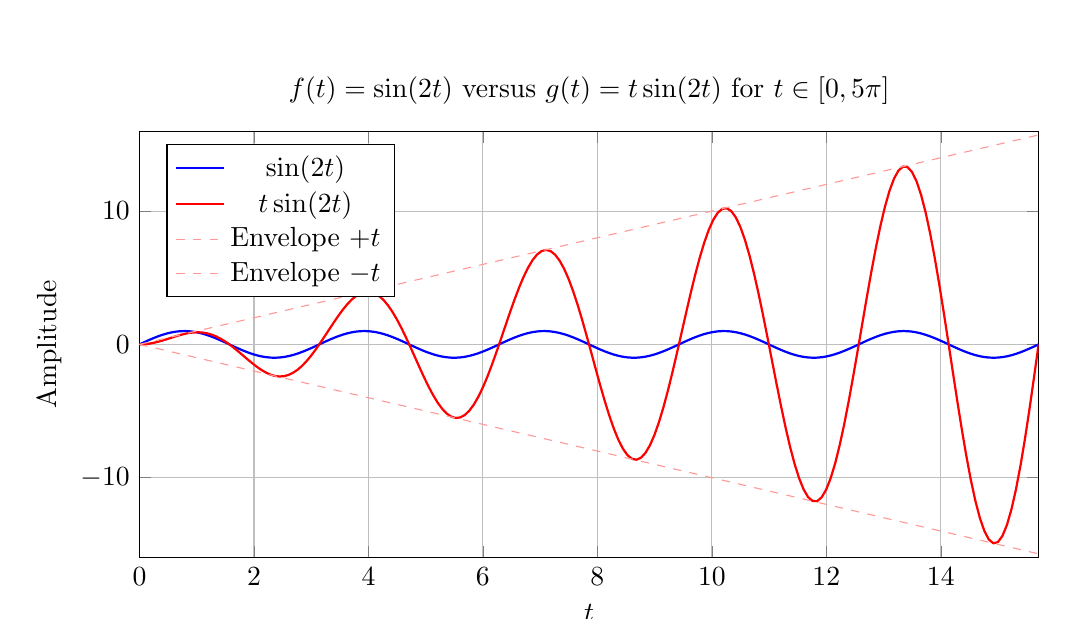
\begin{tikzpicture}
  \begin{axis}[
    xlabel={$t$},
    ylabel={Amplitude},
    xmin=0, xmax=15.708,
    ymin=-16, ymax=16,
    grid=major,
    width=13cm, height=7cm,
    legend pos=north west,
    title={$f(t)=\sin(2t)$ versus $g(t)=t\sin(2t)$ for $t\in[0,5\pi]$}
  ]
    \addplot[blue, thick, domain=0:15.708, samples=200]
      {sin(deg(2*x))};
    \addlegendentry{$\sin(2t)$}
    \addplot[red, thick, domain=0:15.708, samples=200]
      {x*sin(deg(2*x))};
    \addlegendentry{$t\sin(2t)$}
    \addplot[red!40, dashed, domain=0:15.708, samples=100] {x};
    \addlegendentry{Envelope $+t$}
    \addplot[red!40, dashed, domain=0:15.708, samples=100] {-x};
    \addlegendentry{Envelope $-t$}
  \end{axis}
\end{tikzpicture}
\end{center}

\noindent
\textit{Caption:} $t\sin(2t)$ represents a resonance phenomenon --- amplitude
grows linearly with time. The factor $t$ in the time domain corresponds to
differentiation in the s-domain.

% =========================================================
\section{Worked Examples}
% =========================================================

%--- Example 1 ---
\begin{infobox}{Example 1: Find $\mathcal{L}\{t^2\cos(3t)\}$}
We use $\mathcal{L}\{t^2 f(t)\} = F''(s)$ with $f(t)=\cos(3t)$,
$F(s)=s/(s^2+9)$.

\textbf{Step 1 --- First derivative} (quotient rule with $u=s$, $v=s^2+9$):
\[
  F'(s) = \frac{1\cdot(s^2+9)-s\cdot 2s}{(s^2+9)^2}
         = \frac{9-s^2}{(s^2+9)^2}.
\]

\textbf{Step 2 --- Second derivative} (quotient rule again with
$u=9-s^2$, $v=(s^2+9)^2$):
\[
  \frac{d}{ds}(9-s^2)= -2s, \qquad
  \frac{d}{ds}(s^2+9)^2 = 2(s^2+9)\cdot 2s = 4s(s^2+9).
\]
\[
  F''(s)
  = \frac{-2s\,(s^2+9)^2 - (9-s^2)\cdot 4s(s^2+9)}{(s^2+9)^4}
  = \frac{-2s(s^2+9) - 4s(9-s^2)}{(s^2+9)^3}.
\]
Expand the numerator:
\[
  -2s^3-18s - 36s+4s^3 = 2s^3-54s = 2s(s^2-27).
\]
Therefore
\[
  \boxed{\mathcal{L}\{t^2\cos(3t)\} = F''(s) = \frac{2s(s^2-27)}{(s^2+9)^3}.}
\]
\end{infobox}
\begin{learnbox}{What Did We Learn? (Example 1)}
For $t^2 f(t)$ we apply two derivatives of $F(s)$ (with the net sign
$(-1)^2=+1$). The quotient rule must be applied carefully twice; keeping the
intermediate expressions factored avoids arithmetic errors.
\end{learnbox}

%--- Example 2 ---
\begin{infobox}{Example 2: Find $\mathcal{L}\{te^{-2t}\sin(t)\}$}
Two transforms are combined here: the First Shifting Theorem and multiplication
by $t$.

\textbf{Step 1 --- Identify the base function.}
Let $g(t)=t\sin(t)$. We want $\mathcal{L}\{e^{-2t}g(t)\}$.
By the First Shifting Theorem, if $\mathcal{L}\{g(t)\}=G(s)$, then
$\mathcal{L}\{e^{-2t}g(t)\}=G(s+2)$.

\textbf{Step 2 --- Compute $G(s)=\mathcal{L}\{t\sin(t)\}$.}
With $f(t)=\sin(t)$, $F(s)=1/(s^2+1)$:
\[
  F'(s) = \frac{-2s}{(s^2+1)^2}, \qquad
  G(s) = -F'(s) = \frac{2s}{(s^2+1)^2}.
\]

\textbf{Step 3 --- Apply the shift $s \to s+2$.}
\[
  \mathcal{L}\{te^{-2t}\sin(t)\} = G(s+2)
  = \frac{2(s+2)}{\bigl((s+2)^2+1\bigr)^2}
  = \frac{2(s+2)}{(s^2+4s+5)^2}.
\]
Therefore
\[
  \boxed{\mathcal{L}\{te^{-2t}\sin(t)\} = \frac{2(s+2)}{(s^2+4s+5)^2}.}
\]
\end{infobox}
\begin{learnbox}{What Did We Learn? (Example 2)}
When $e^{at}$ and a $t$-factor both appear, first use multiplication by $t$ to
find $G(s)$, then shift $s \to s-a$ (here $s \to s+2$). The two properties
compose neatly.
\end{learnbox}

%--- Example 3 ---
\begin{infobox}{Example 3: Given $\mathcal{L}\{f(t)\}=\ln(s^2+a^2)$, find $\mathcal{L}\{tf(t)\}$}
We use $\mathcal{L}\{tf(t)\}=-F'(s)$ with $F(s)=\ln(s^2+a^2)$.

\textbf{Differentiate $F(s)$:}
\[
  F'(s) = \frac{d}{ds}\ln(s^2+a^2) = \frac{2s}{s^2+a^2}.
\]

\textbf{Apply the formula:}
\[
  \mathcal{L}\{tf(t)\} = -F'(s) = -\frac{2s}{s^2+a^2}.
\]

\textbf{Pedagogical Note:} In rigorous transform theory, a valid Laplace transform of an exponential-order function must satisfy $\lim_{s \to \infty} F(s) = 0$. Because $\lim_{s \to \infty} \ln(s^2+a^2) = \infty$, no classical function possesses $\ln(s^2+a^2)$ as its standard Laplace transform. However, this problem is a standard formal operational exercise in transform calculus to practice applying the differentiation rule $\mathcal{L}\{tf(t)\} = -F'(s)$ algebraically.
\end{infobox}
\begin{learnbox}{What Did We Learn? (Example 3)}
The multiplication-by-$t$ formula works purely algebraically on any differentiable $F(s)$ --- only $F'(s)$ needs to be computed. Here $F(s)=\ln(s^2+a^2)$ differentiates easily by the chain rule to give $-2s/(s^2+a^2)$.
\end{learnbox}

% =========================================================
\section{Extended Standard Table}
% =========================================================
\begin{center}
\begin{tabular}{@{}l l@{}}
\toprule
\textbf{$f(t)$} & \textbf{$\mathcal{L}\{f(t)\} = F(s)$} \\
\midrule
$t$ & $\dfrac{1}{s^2}$ \\[6pt]
$t^2$ & $\dfrac{2}{s^3}$ \\[6pt]
$t^n$ & $\dfrac{n!}{s^{n+1}}$ \\[6pt]
$te^{at}$ & $\dfrac{1}{(s-a)^2}$ \\[6pt]
$t^n e^{at}$ & $\dfrac{n!}{(s-a)^{n+1}}$ \\[6pt]
$t\sin(at)$ & $\dfrac{2as}{(s^2+a^2)^2}$ \\[6pt]
$t\cos(at)$ & $\dfrac{s^2-a^2}{(s^2+a^2)^2}$ \\[6pt]
$t\sinh(at)$ & $\dfrac{2as}{(s^2-a^2)^2}$ \\[6pt]
$t\cosh(at)$ & $\dfrac{s^2+a^2}{(s^2-a^2)^2}$ \\[6pt]
\bottomrule
\end{tabular}
\end{center}

\noindent
(All entries for $t\cosh$ and $t\sinh$ are derived using
$\mathcal{L}\{\sinh(at)\}=a/(s^2-a^2)$ and
$\mathcal{L}\{\cosh(at)\}=s/(s^2-a^2)$ via the same quotient rule.)

% =========================================================
\section{Excel Example}
% =========================================================
\subsection*{Numerical Verification of $\mathcal{L}\{t\sin(t)\}$ at $s=2$}

The exact value is
\[
  \mathcal{L}\{t\sin(t)\}\big|_{s=2}
  = \frac{2s}{(s^2+1)^2}\bigg|_{s=2}
  = \frac{4}{25} = 0.16.
\]

We approximate the integral numerically using the trapezoid rule with step
$h=0.1$ from $t=0$ to $t=8$.

\begin{center}
\begin{tabular}{@{}c c c c@{}}
\toprule
\textbf{Column A} & \textbf{Column B} & \textbf{Column C}
                  & \textbf{Remark} \\
$t$ & $e^{-2t}\cdot t\sin(t)$ & Cumulative Trapezoid Sum & \\
\midrule
0.0 & \texttt{=EXP(-2*A2)*A2*SIN(A2)} = 0.000000 &
  0.000000 & Initial value \\
0.1 & \texttt{=EXP(-2*A3)*A3*SIN(A3)} = 0.008181 &
  \texttt{=C2+(B2+B3)/2*0.1} = 0.000409 & Trapezoid step 1 \\
0.2 & \texttt{=EXP(-2*A4)*A4*SIN(A4)} = 0.026889 &
  \texttt{=C3+(B3+B4)/2*0.1} = 0.002162 & Trapezoid step 2 \\
\bottomrule
\end{tabular}
\end{center}

\textbf{Spreadsheet setup instructions:}
\begin{enumerate}
  \item Enter $t$ values in Column A: cell A2 = 0, A3 = 0.1, A4 = 0.2,
        \ldots, A82 = 8.0. Use fill-down.
  \item Column B formula (enter in B2, fill to B82):
        \texttt{=EXP(-2*A2)*A2*SIN(A2)}
  \item Column C (cumulative trapezoid sum):
        C2 = 0,\quad C3 = \texttt{=C2+(B2+B3)/2*0.1},\quad fill to C82.
  \item Final approximation: value in cell C82.
\end{enumerate}

\begin{learnbox}{Excel vs Exact Value}
With $h=0.1$ the trapezoid rule gives approximately $\approx 0.1598$ at $t=8$.
The exact value is $0.16$. The agreement to three significant figures confirms
both the formula and the numerical method. Reducing $h$ to $0.01$ or extending
to $t=12$ brings the approximation even closer to $0.16$.
\end{learnbox}

% =========================================================
\section{Python Example}
% =========================================================
\begin{lstlisting}[language=Python, caption={Symbolic verification of multiplication-by-$t$ property using SymPy}]
import sympy as sp

s, t, a, n = sp.symbols('s t a n', positive=True)

# --- Case 1: f(t) = sin(at) ---
F_sin = sp.laplace_transform(sp.sin(a*t), t, s, noconds=True)
print("L{sin(at)} =", F_sin)          # a/(s**2 + a**2)
neg_dF_sin = -sp.diff(F_sin, s)
neg_dF_sin_simplified = sp.simplify(neg_dF_sin)
print("-d/ds L{sin(at)} =", neg_dF_sin_simplified)
# Expected: 2*a*s/(s**2 + a**2)**2

# Verify against direct transform of t*sin(at)
L_tsin = sp.laplace_transform(t*sp.sin(a*t), t, s, noconds=True)
print("L{t*sin(at)} =", sp.simplify(L_tsin))
# Expected: 2*a*s/(s**2 + a**2)**2
print("Match:", sp.simplify(neg_dF_sin - L_tsin) == 0)   # True

print()

# --- Case 2: f(t) = e^(at) ---
F_exp = sp.laplace_transform(sp.exp(a*t), t, s, noconds=True)
print("L{e^(at)} =", F_exp)            # 1/(-a + s)
neg_dF_exp = sp.simplify(-sp.diff(F_exp, s))
print("-d/ds L{e^(at)} =", neg_dF_exp)
# Expected: 1/(s - a)**2

L_texp = sp.laplace_transform(t*sp.exp(a*t), t, s, noconds=True)
print("L{t*e^(at)} =", sp.simplify(L_texp))
# Expected: 1/(s - a)**2
print("Match:", sp.simplify(neg_dF_exp - L_texp) == 0)   # True

print()

# --- Case 3: f(t) = cos(at) ---
F_cos = sp.laplace_transform(sp.cos(a*t), t, s, noconds=True)
print("L{cos(at)} =", F_cos)           # s/(s**2 + a**2)
neg_dF_cos = sp.simplify(-sp.diff(F_cos, s))
print("-d/ds L{cos(at)} =", neg_dF_cos)
# Expected: (s**2 - a**2)/(s**2 + a**2)**2

L_tcos = sp.laplace_transform(t*sp.cos(a*t), t, s, noconds=True)
print("L{t*cos(at)} =", sp.simplify(L_tcos))
# Expected: (s**2 - a**2)/(s**2 + a**2)**2
print("Match:", sp.simplify(neg_dF_cos - L_tcos) == 0)   # True

print()

# --- General formula for t^n * e^(at), n = 1, 2, 3 ---
F_e = 1/(s - a)   # L{e^(at)}
for k in [1, 2, 3]:
    Fn = ((-1)**k) * sp.diff(F_e, s, k)
    print(f"L{{t^{k} * e^(at)}} = {sp.simplify(Fn)}")
# Expected:
# L{t^1 * e^(at)} =  1/(s - a)**2
# L{t^2 * e^(at)} =  2/(s - a)**3
# L{t^3 * e^(at)} =  6/(s - a)**4
\end{lstlisting}

\begin{learnbox}{What Did We Learn? (Python)}
SymPy's \texttt{laplace\_transform} and \texttt{diff} confirm all the
multiplication-by-$t$ results symbolically. The loop over $n=1,2,3$ shows the
pattern $n!/(s-a)^{n+1}$ emerging automatically. Symbolic verification is a
powerful sanity check before applying these results numerically.
\end{learnbox}

% =========================================================
\section{Viva-Style Oral Questions}
% =========================================================
\begin{enumerate}

\item \textbf{State the multiplication-by-$t$ formula.}\\
\textit{Answer.} If $\mathcal{L}\{f(t)\}=F(s)$, then
$\mathcal{L}\{tf(t)\}=-F'(s)=-dF/ds$.

\item \textbf{How is the formula proved?}\\
\textit{Answer.} Start from $F(s)=\int_0^\infty e^{-st}f(t)\,dt$. Differentiate
both sides with respect to $s$. By the Leibniz rule (differentiation under the
integral sign), the derivative passes inside the integral and $\partial/\partial
s\,[e^{-st}]=-te^{-st}$. This gives $F'(s)=-\mathcal{L}\{tf(t)\}$, hence
$\mathcal{L}\{tf(t)\}=-F'(s)$.

\item \textbf{Where does the $(-1)^n$ factor come from in the general formula?}\\
\textit{Answer.} Each differentiation with respect to $s$ brings out one factor
of $(-t)$ from $e^{-st}$. After $n$ differentiations, the cumulative factor is
$(-t)^n=(-1)^n t^n$. Moving $(-1)^n$ outside the integral gives the sign factor
in $(-1)^n d^n F/ds^n$.

\item \textbf{What is $\mathcal{L}\{t\sin(at)\}$?}\\
\textit{Answer.} $\mathcal{L}\{t\sin(at)\}=2as/(s^2+a^2)^2$. This follows from
differentiating $F(s)=a/(s^2+a^2)$ with the quotient rule and negating.

\item \textbf{What is $\mathcal{L}\{t\cos(at)\}$?}\\
\textit{Answer.} $\mathcal{L}\{t\cos(at)\}=(s^2-a^2)/(s^2+a^2)^2$. Differentiate
$F(s)=s/(s^2+a^2)$ via the quotient rule: $F'(s)=(a^2-s^2)/(s^2+a^2)^2$; then
negate.

\item \textbf{How do you handle a function like $te^{-3t}\cos(2t)$?}\\
\textit{Answer.} Two steps: (i) find $G(s)=\mathcal{L}\{t\cos(2t)\}=(s^2-4)/(s^2+4)^2$
using multiplication by $t$; (ii) apply the First Shifting Theorem with $a=-3$
to replace $s$ by $s+3$: $G(s+3)=((s+3)^2-4)/((s+3)^2+4)^2$.

\item \textbf{What is the physical interpretation of $t\sin(\omega t)$?}\\
\textit{Answer.} $t\sin(\omega t)$ represents a resonance phenomenon in which the
amplitude of oscillation grows linearly with time. In control systems and
vibrations, this corresponds to the response of a system driven at its natural
frequency $\omega$ with no damping --- energy builds up indefinitely.

\item \textbf{What is the general result for $\mathcal{L}\{t^n e^{at}\}$?}\\
\textit{Answer.} $\mathcal{L}\{t^n e^{at}\}=n!/(s-a)^{n+1}$. It follows from
applying the general formula $(-1)^n d^n/ds^n$ to $F(s)=1/(s-a)$ and computing
$F^{(n)}(s)=(-1)^n n!/(s-a)^{n+1}$.

\end{enumerate}

% =========================================================
\section{Descriptive Questions}
% =========================================================
\begin{enumerate}

\item \textbf{Prove the multiplication-by-$t$ formula
$\mathcal{L}\{tf(t)\}=-F'(s)$.}\\
\textit{Answer.} Define $F(s)=\int_0^\infty e^{-st}f(t)\,dt$. Differentiate
both sides with respect to $s$, invoking the Leibniz rule to move the derivative
inside the integral (valid when $f$ is of exponential order and piecewise
continuous):
\[
  F'(s)=\int_0^\infty \frac{\partial}{\partial s}[e^{-st}]f(t)\,dt
  =\int_0^\infty(-t)e^{-st}f(t)\,dt = -\mathcal{L}\{tf(t)\}.
\]
Rearranging gives $\mathcal{L}\{tf(t)\}=-F'(s)$. $\square$

\item \textbf{Prove the general formula
$\mathcal{L}\{t^n f(t)\}=(-1)^n F^{(n)}(s)$.}\\
\textit{Answer.} Proceed by induction. Base case $n=1$ is proved above. Assume
$\mathcal{L}\{t^{k}f(t)\}=(-1)^k F^{(k)}(s)$ holds. Let
$g(t)=t^k f(t)$, $G(s)=(-1)^k F^{(k)}(s)$. By the $n=1$ result,
\[
  \mathcal{L}\{t^{k+1}f(t)\}=\mathcal{L}\{t\cdot g(t)\}
  =-G'(s)=-(-1)^k F^{(k+1)}(s)=(-1)^{k+1}F^{(k+1)}(s).
\]
This completes the induction. $\square$

\item \textbf{Find $\mathcal{L}\{t^2\sin(at)\}$ completely.}\\
\textit{Answer.} We need $(-1)^2 F''(s)=F''(s)$ with $F(s)=a/(s^2+a^2)$.

First derivative (quotient rule):
$F'(s) = -2as/(s^2+a^2)^2.$

Second derivative: let $u=-2as$, $v=(s^2+a^2)^2$.
$u'=-2a$, $v'=4s(s^2+a^2)$.
\[
F''(s)=\frac{-2a(s^2+a^2)^2-(-2as)\cdot 4s(s^2+a^2)}{(s^2+a^2)^4}
= \frac{-2a(s^2+a^2)+8as^2}{(s^2+a^2)^3}
= \frac{2a(3s^2-a^2)}{(s^2+a^2)^3}.
\]
Therefore $\mathcal{L}\{t^2\sin(at)\}=\dfrac{2a(3s^2-a^2)}{(s^2+a^2)^3}.$

\item \textbf{Find $\mathcal{L}\{te^{-t}\cos(2t)\}$.}\\
\textit{Answer.} Step 1: find $G(s)=\mathcal{L}\{t\cos(2t)\}$.
With $F(s)=s/(s^2+4)$, quotient rule gives
$F'(s)=(4-s^2)/(s^2+4)^2$, so
$G(s)=-F'(s)=(s^2-4)/(s^2+4)^2$.

Step 2: shift $s\to s+1$ (First Shifting Theorem with $a=-1$):
\[
  \mathcal{L}\{te^{-t}\cos(2t)\}=G(s+1)=\frac{(s+1)^2-4}{((s+1)^2+4)^2}
  =\frac{s^2+2s-3}{(s^2+2s+5)^2}.
\]

\item \textbf{Derive $\mathcal{L}\{t^n\}$ using the multiplication-by-$t$ property
and $\mathcal{L}\{1\}=1/s$.}\\
\textit{Answer.} Let $f(t)=1$, $F(s)=1/s$. Apply the general formula:
\[
  \frac{d^n}{ds^n}\left(\frac{1}{s}\right)
  = \frac{(-1)^n n!}{s^{n+1}}.
\]
Therefore
\[
  \mathcal{L}\{t^n\}=(-1)^n\cdot\frac{(-1)^n n!}{s^{n+1}}=\frac{n!}{s^{n+1}}.
\]
This matches the known result for $\mathcal{L}\{t^n\}$, confirming the formula.

\end{enumerate}

% =========================================================
\section{Practice Problems}
% =========================================================
\begin{enumerate}

\item Find $\mathcal{L}\{t\cosh(2t)\}$.\\
\textit{Hint:} Differentiate $F(s)=s/(s^2-4)$; apply quotient rule;
negate. \textit{Answer:} $(s^2+4)/(s^2-4)^2$.

\item Find $\mathcal{L}\{t^2\sin(t)\}$.\\
\textit{Hint:} Use $F''(s)$ with $F(s)=1/(s^2+1)$; differentiate twice.
\textit{Answer:} $2(3s^2-1)/(s^2+1)^3$.

\item Find $\mathcal{L}\{te^{3t}\cos(t)\}$.\\
\textit{Hint:} First compute $G(s)=\mathcal{L}\{t\cos(t)\}=(s^2-1)/(s^2+1)^2$;
then shift $s\to s-3$.
\textit{Answer:} $((s-3)^2-1)/((s-3)^2+1)^2$.

\item Find $\mathcal{L}\{t^3 e^{-2t}\}$.\\
\textit{Hint:} Use $\mathcal{L}\{t^n e^{at}\}=n!/(s-a)^{n+1}$ with $n=3$, $a=-2$.
\textit{Answer:} $6/(s+2)^4$.

\item Find $\mathcal{L}\{t\sinh(3t)\}$.\\
\textit{Hint:} Differentiate $F(s)=3/(s^2-9)$; negate.
\textit{Answer:} $6s/(s^2-9)^2$.

\item Given $\mathcal{L}\{f(t)\}=\arctan(1/s)$, find $\mathcal{L}\{tf(t)\}$.\\
\textit{Hint:} Differentiate $F(s)=\arctan(1/s)$ using chain rule:
$dF/ds = \frac{1}{1+(1/s)^2}\cdot(-1/s^2) = -1/(s^2+1)$. Negate.
\textit{Answer:} $1/(s^2+1)$.

\end{enumerate}

% =========================================================
\section{MCQs}
% =========================================================
\begin{enumerate}

\item If $\mathcal{L}\{f(t)\}=F(s)$, then $\mathcal{L}\{t^n f(t)\}$ equals

(a) $(-1)^n F(s)$\quad
(b) $(-1)^n F^{(n)}(s)$\quad
(c) $n!\,F(s)$\quad
(d) $F^{(n)}(s)$

\textbf{Correct answer: (b).}\\
\textit{Explanation:} Each differentiation with respect to $s$ produces a factor
of $(-t)$; after $n$ steps the sign factor is $(-1)^n$.

\item The transform $\mathcal{L}\{t\sin(at)\}$ is

(a) $\dfrac{a}{(s^2+a^2)^2}$\quad
(b) $\dfrac{2as}{(s^2+a^2)^2}$\quad
(c) $\dfrac{s}{s^2+a^2}$\quad
(d) $\dfrac{2a}{s^2+a^2}$

\textbf{Correct answer: (b).}\\
\textit{Explanation:} Differentiate $a/(s^2+a^2)$ and negate;
quotient rule gives $-(-2as)/(s^2+a^2)^2=2as/(s^2+a^2)^2$.

\item $\mathcal{L}\{te^{at}\}$ equals

(a) $\dfrac{1}{s-a}$\quad
(b) $\dfrac{a}{(s-a)^2}$\quad
(c) $\dfrac{1}{(s-a)^2}$\quad
(d) $\dfrac{1}{(s+a)^2}$

\textbf{Correct answer: (c).}\\
\textit{Explanation:} Differentiate $F(s)=1/(s-a)$ to get $-1/(s-a)^2$; negate
to obtain $1/(s-a)^2$.

\item To apply the multiplication-by-$t$ property, you differentiate with
respect to

(a) $t$\quad
(b) $a$\quad
(c) $s$\quad
(d) $\omega$

\textbf{Correct answer: (c).}\\
\textit{Explanation:} The property is derived by differentiating $F(s)$ with
respect to the frequency variable $s$, not with respect to $t$.

\item Using $\mathcal{L}\{1\}=1/s$, the transform $\mathcal{L}\{t^2\}$ via
the multiplication-by-$t$ formula is

(a) $\dfrac{1}{s^2}$\quad
(b) $\dfrac{1}{s^3}$\quad
(c) $\dfrac{2}{s^3}$\quad
(d) $\dfrac{2}{s^2}$

\textbf{Correct answer: (c).}\\
\textit{Explanation:} $F(s)=1/s$; $F''(s)=2/s^3$;
$\mathcal{L}\{t^2\}=(-1)^2 F''(s)=2/s^3$.

\end{enumerate}

% =========================================================
\section{Common Mistakes}
% =========================================================
\begin{mistakebox}{Common Mistakes in Multiplication by $t$}
\begin{tabular}{@{}p{4cm} p{5cm} p{5cm}@{}}
\toprule
\textbf{Mistake} & \textbf{What Students Do} & \textbf{Correct Approach} \\
\midrule
Differentiate w.r.t.\ $t$ instead of $s$ &
  Compute $d/dt[f(t)]$ and use that as the transformed result &
  Always differentiate $F(s)$ with respect to $s$, never touch $f(t)$ \\
Forget the $(-1)^n$ sign &
  Write $\mathcal{L}\{t^n f\} = F^{(n)}(s)$ without the sign factor;
  get wrong signs for odd $n$ &
  Include $(-1)^n$; for $n=1$ the answer is $-F'(s)$, not $+F'(s)$ \\
Apply formula without $n$ derivatives &
  Differentiate once even when computing $\mathcal{L}\{t^2 f\}$,
  stopping at $F'(s)$ instead of $F''(s)$ &
  For $t^n f(t)$ differentiate $F(s)$ exactly $n$ times \\
Sign error in quotient rule &
  Mix up numerator terms when differentiating rational $F(s)$;
  e.g.\ write $F'(s) = (u'v + uv')/v^2$ instead of $(u'v - uv')/v^2$ &
  Quotient rule: $F'(s) = (u'v - uv')/v^2$; write out $u,v,u',v'$
  explicitly before substituting \\
Use $+F'(s)$ for $\mathcal{L}\{tf(t)\}$ &
  Write $\mathcal{L}\{tf(t)\} = +F'(s)$, forgetting the negative sign &
  The formula is $\mathcal{L}\{tf(t)\} = -F'(s)$; the minus sign
  comes from $\partial/\partial s[e^{-st}] = -te^{-st}$ \\
\bottomrule
\end{tabular}
\end{mistakebox}

% =========================================================
\section{Quick Recap}
% =========================================================
\begin{learnbox}{Quick Recap --- Multiplication by $t$}
\begin{itemize}
  \item \textbf{Main formula:}
        $\mathcal{L}\{tf(t)\} = -F'(s)$, where $F(s)=\mathcal{L}\{f(t)\}$.
  \item \textbf{General formula:}
        $\mathcal{L}\{t^n f(t)\} = (-1)^n\,\dfrac{d^n}{ds^n}F(s)$;
        the sign alternates with $n$.
  \item \textbf{Key results:}
        $\mathcal{L}\{te^{at}\} = 1/(s-a)^2$;\quad
        $\mathcal{L}\{t\sin(at)\} = 2as/(s^2+a^2)^2$;\quad
        $\mathcal{L}\{t\cos(at)\} = (s^2-a^2)/(s^2+a^2)^2$.
  \item \textbf{Resonance interpretation:}
        $t\sin(\omega t)$ has linearly growing amplitude --- this is the
        mathematical signature of an undamped resonance; its transform
        $2\omega s/(s^2+\omega^2)^2$ encodes that growth in the s-domain.
  \item \textbf{Extended standard table:}
        Use the table in Section~8 for rapid lookup of $t\sinh$, $t\cosh$,
        $t^n e^{at}$, $t^n$ without re-deriving.
  \item \textbf{Combined $e^{at}\cdot t\cdot f(t)$:}
        First apply multiplication by $t$ to get $G(s)$, then shift
        $s\to s-a$ by the First Shifting Theorem.
  \item \textbf{Sign discipline:}
        Always write out $u, v, u', v'$ in the quotient rule before
        substituting; this prevents the most common sign errors.
  \item \textbf{Verification:}
        Cross-check with SymPy (\texttt{sp.diff(F,s)}) or the extended
        table; numerical Excel integration confirms to 3--4 significant
        figures for reasonable step sizes.
\end{itemize}
\end{learnbox}

\end{document}
